\section{Methods}

\subsection{Creating a representative dataset of questions}
\label{creating_dataset}

As shown in \Cref{questions_objective}, our codebase requires the creation of a new dataset of questions with three main properties.

\begin{enumerate}
	\item Questions should have short an unambiguous answers. \label{q_short}
	\item They must cover a large set of topics, eras, and places. \label{q_widespread}
	\item They must allow for the creation of sensible counterfactuals by having sets of questions with the same answer format. \label{q_counterfactual}
\end{enumerate}

To address Items 1 and 3, we follow the approach done by \citeauthor{factual_recall} in creating questions which have a question with a particular ``object'' as its nucleus.
This way, it's possible to create counterfactuals that have the same format of the original answer by randomly sampling from the set of answers, as shown in \cref{counterparametric_table}.

\begin{table}[h]
	\newcommand{\vwidth}[1]{\begin{minipage}[t][][t]{38ex}\ttfamily #1\end{minipage}}
	\newcommand{\rep}[1]{{\setlength{\fboxsep}{0pt}\fcolorbox{Gray}{Gray!80}{\textit{#1}}}}

	\centering
	\scriptsize

	\begin{tabularx}{\textwidth}{>{\ttfamily}l@{\hspace{4pt}}|>{\ttfamily}l@{\hspace{4pt}}>{\ttfamily}l@{\hspace{4pt}}>{\ttfamily}l@{\hspace{12pt}}>{\ttfamily}X}
		\toprule
			\rmfamily \bfseries Base Question & \rmfamily \bfseries Object & \rmfamily \bfseries \parbox{40pt}{Parametric \\ Answer} & \rmfamily \bfseries \parbox{50pt}{Counterparametric Answer} & \rmfamily \bfseries \parbox{100pt}{Question with counterparametric context} \\
		\midrule
			\multirow{6}{65pt}[-100pt]{Q: What is the date of birth of \protect\rep{\{person\}}? \\ A: The date of birth of \protect\rep{\{person\}} is} & \textcolor{Red}{Che~Guevara} &  \textcolor{Red}{June~14,~1928} & \textcolor{Apricot}{965~AD} & \vwidth{Context: [the date of birth of \textcolor{Red}{Che~Guevara} is \textcolor{Apricot}{965~AD}]. \\ Q: What is the date of birth of \textcolor{Red}{Che~Guevara}? \\ A: The date of birth of \textcolor{Red}{Che~Guevara} is} \vspace{4pt} \\
			& \textcolor{Apricot}{Ibn~al-Haytham} &  \textcolor{Apricot}{965~AD} & \textcolor{Red}{June~14,~1928} & \vwidth{Context: [the date of birth of \textcolor{Apricot}{Ibn~al-Haytham} is \textcolor{Red}{June~14,~1928}]. \\ Q: What is the date of birth of \textcolor{Apricot}{Ibn~al-Haytham}? \\ A: The date of birth of \textcolor{Apricot}{Ibn~al-Haytham} is} \vspace{4pt} \\
			& \textcolor{Blue}{Boyan~Slat} &  \textcolor{Blue}{27~January~1994} & \textcolor{Brown}{February~23,~1868} & \vwidth{Context: [the date of birth of \textcolor{Blue}{Boyan~Slat} is \textcolor{Brown}{February~23,~1868}]. \\ Q: What is the date of birth of \textcolor{Blue}{Boyan~Slat}? \\ A: The date of birth of \textcolor{Blue}{Boyan~Slat} is} \vspace{4pt} \\
			& \textcolor{Brown}{W.E.B~Du~Bois} &  \textcolor{Brown}{February~23,~1868} & \textcolor{Red}{June~14,~1928} & \vwidth{Context: [the date of birth of \textcolor{Brown}{W.E.B~Du~Bois} is \textcolor{Red}{June~14,~1928}]. \\ Q: What is the date of birth of \textcolor{Brown}{W.E.B~Du~Bois}? \\ A: The date of birth of \textcolor{Brown}{W.E.B~Du~Bois} is} \vspace{4pt} \\
			% & \textcolor{Cerulean}{Stephen~Hawking} &  \textcolor{Cerulean}{January~8,~1942} & \textcolor{Apricot}{965~AD} & \vwidth{Context: [the date of birth of \textcolor{Cerulean}{Stephen~Hawking} is \textcolor{Apricot}{965~AD}]. \\ Q: What is the date of birth of \textcolor{Cerulean}{Stephen~Hawking}? \\ A: The date of birth of \textcolor{Cerulean}{Stephen~Hawking} is} \vspace{4pt} \\
			% & \textcolor{DarkOrchid}{Shirin~Ebadi} &  \textcolor{DarkOrchid}{June~21,~1947} & \textcolor{Red}{June~14,~1928} & \vwidth{Context: [the date of birth of \textcolor{DarkOrchid}{Shirin~Ebadi} is \textcolor{Red}{June~14,~1928}]. \\ Q: What is the date of birth of \textcolor{DarkOrchid}{Shirin~Ebadi}? \\ A: The date of birth of \textcolor{DarkOrchid}{Shirin~Ebadi} is} \vspace{2pt} \\
		\bottomrule
	\end{tabularx}
	% \caption{Example of the sampling done to produce counterparametric answers. Counterparametric answers are generated by sampling a random answer from the parametric answers from the same base questions; to ensure that no parametric and counterparametric pair are identical, we only sample between different parametric answers. Note that the same parametric answer can appear several times as a counterparametric in different questions.}
	\caption{Using the same question format allows us to repurpose previous parametric answers as counterparametric ones.}
	\label{counterparametric_table}
\end{table}

\vspace{1em} To address Item 2, we manually create a large of different topics, questions, and objects referred to that question in various categories.
To create the questions that are being queries, every question is matched to an object of its corresponding category as shown in \cref{source_data_example}.

\begin{table}[h]
	\setlength{\fboxsep}{0pt}
	\setlength{\fboxrule}{1pt}
	\newcommand{\rep}[1]{{\setlength{\fboxsep}{0pt}\fcolorbox{Gray}{Gray!80}{\textit{#1}}}}

	\centering
	\scriptsize
	\begin{tabular}{>{\bfseries}c | l | c | l}
		\toprule
			\bfseries Category & \bfseries Base Questions & \bfseries Object & \bfseries Final Questions \\
		\midrule
			Person & \begin{minipage}{.30\textwidth}
				\ttfamily
				Q: What is the date of birth of \rep{\{person\}}? \\ A: The date of birth of \rep{\{person\}} is \\[1ex]
				Q: In what city was \rep{\{person\}} born? \\ A: \rep{\{person\}} was born in
			\end{minipage} &
			\begin{minipage}{.12\textwidth}
				\ttfamily
				\fcolorbox{Gray!50}{Gray!50}{\textcolor{Red}{Che~Guevara}} \\[1ex]
				\fcolorbox{Gray!50}{Gray!50}{\textcolor{Sepia}{Confucius}}
			\end{minipage} &
			\begin{minipage}{.40\textwidth}
				\ttfamily
				Q: What is the date of birth of \textcolor{Red}{Che~Guevara}? \\ A: The date of birth of \textcolor{Red}{Che~Guevara} is \\[1ex]
				Q: What is the date of birth of \textcolor{Sepia}{Confucius}? \\ A: The date of birth of \textcolor{Sepia}{Confucius} is \\[1ex]
				Q: In what city was \textcolor{Red}{Che~Guevara} born? \\ A: \textcolor{Red}{Che~Guevara} was born in \\[1ex]
				Q: In what city was \textcolor{Sepia}{Confucius} born? \\ A: \textcolor{Sepia}{Confucius} was born in
			\end{minipage} \\
		\midrule
			City & \begin{minipage}{.30\textwidth}
				\ttfamily
				Q: What country is \rep{\{city\}} in? \\ A: \rep{\{city\}} is in
			\end{minipage} &
			\begin{minipage}{.10\textwidth}
				\ttfamily
				\fcolorbox{Gray!50}{Gray!50}{\textcolor{BurntOrange}{Cairo}} \\[1ex]
				\fcolorbox{Gray!50}{Gray!50}{\textcolor{ForestGreen}{Mumbai}}
			\end{minipage} &
			\begin{minipage}{.40\textwidth}
				\ttfamily
				Q: What country is \textcolor{BurntOrange}{Cairo} in? \\ A: \textcolor{BurntOrange}{Cairo} is in \\[1ex]
				Q: What country is \textcolor{ForestGreen}{Mumbai} in? \\ A: \textcolor{ForestGreen}{Mumbai} is in
			\end{minipage} \\
		\bottomrule
	\end{tabular}
	\caption{Some examples of the base-question and object generation that are fed to the models for finding parametric answers.}
	\label{source_data_example}
\end{table}

In addition to having the previous properties, it's easy to make a long list of questions using this method.

\subsection{When does a model choose the provided context knowledge over its inherent knowledge?}

\subsubsection{Model Selection}

In order to get a general understanding of large language models with added context, we test the queries generated in \cref{creating_dataset} into models of different types and sizes.

\begin{table}[h]
	\centering
	\begin{tabular}{>{\bfseries}c@{\hspace{20pt}}l l}
		\toprule
			& \bfseries Seq2Seq Model & \bfseries Decoder-Only Model \\
		\midrule
			Small & \ttfamily Flan-T5-XL & \ttfamily Meta-Llama-3.1-8B-Instruct \\
			Large & \ttfamily Flan-T5-XXL & \ttfamily Meta-Llama-3.1-70B-Instruct \\
		\bottomrule
	\end{tabular}
	\caption{The four large language models chosen for this research.}
\end{table}

The Flan-T5 models \citep{flant5} are an extension to the original Seq2Seq T5 models \citep{t5} which are fine-tuned to particular NLP tasks framed as text-to-text problems.
Compared to T5, it's generally better at following instructions and has improved zero-shot performance.

The Llama models \citep{llama3} are Decoder-only models with a dense transformer architecture that are fine-tuned for instruction-following tasks, and are specially adept at complex prompts.

\subsubsection{What type of answer does each model select for each question?}

TODO: Maybe I should explain the whole drama with the counterparamteric answers here.

\begin{figure}[h]
	\centering
	\fbox{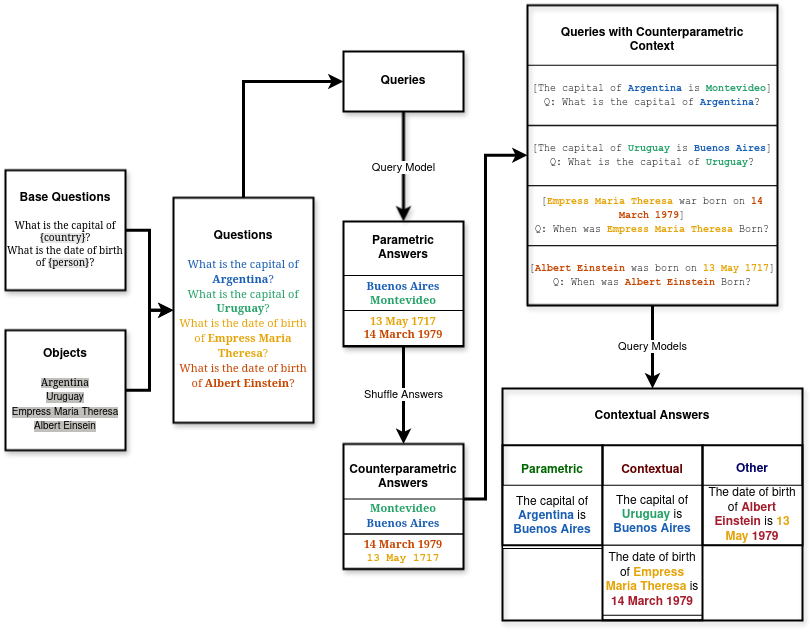
\includegraphics[width=.75\textwidth]{Method.png}}
	\caption{Example diagram of steps used to calculate the two sets of answers, \textit{parametric} and \textit{contextual}, and to compare them to answer the question in this objective. Many of the terms in this diagram are explained in the \hyperref[glossary]{Glossary}.}
\end{figure}

To ensure that the results are simple to interpret and minimise the chance that the result is affected by randomness, once we select the queries we follow the example of \citeauthor{ragged} and use Greedy Decoding to find the answer.

While beam search with a short beam width tends to produce more accurate results for long answers \citep{sutskever_seq2seqlearning,wu_mltranslation} and there are many other sampling methods that produce better results \citep{text_degeneration}, this is likely to not have an effect on experiments that result in shorter answers \citep{t5}.

\subsection{Can we use the perplexity score of an answer to predict whether it came from inherent or contextual knowledge?}

\subsubsection{Perplexity Score}

The Perplexity score of an answer is normally used to measure the inverse of the certainty that the model has of a particular answer \citep{fewshotlearners,retro}.
In a sense, it's the ``surprise'' of a model that a certain answer is correct.

We can define the probability of model $Q$ choosing a token $x_n$ with context $x_1, \dots, x_{n - 1}$ by calculating the softmax value of all the logits for the possible words for this token.

This probability of the tokens corresponding to a particular answer $x_1, \dots, x_n$ can be accumulated to calculate the negative log-likelihood NLL, which is used to calculate the perplexity PPL using the formulas from \cref{eq:nll,eq:ppl}.

\begin{align}
	\text{NLL} \left( x_1, \dots, x_n \mid Q \right) &= - \frac{1}{n} \sum^n_{i = 1} \log_2 P \left( x_i \mid Q, x_1, \dots, x_{i - 1} \right) \label{eq:nll} \\
	\text{PPL} \left( x_1, \dots, x_n \mid Q \right) &= {2 ^ {\text{NLL} \left( x_1, \dots, x_n \mid Q \right)}} \label{eq:ppl}
\end{align}

\subsubsection{Perplexity of the parametric answer with counterfactual context and vice-versa}

Note that the token $x_n$ does not necessarily have to be the result of applying the query $x_1, \dots, x_{n - 1}$ to a model.
We can instead use teacher-forcing \citep{teacher_forcing} to calculate the perplexity values of finding the parametric answer in the query with counterfactual context, and the 
